\documentclass{article}

\usepackage[utf8]{inputenc}
\usepackage[T1]{fontenc}
\usepackage[norsk,english]{babel}   %Norsk først så engelsk, så engelsk blir prioritert
\usepackage{graphicx}
\usepackage{amsmath}        %For å kunne skrive matte
\usepackage{listings}       %For å kunne skrive inn kode med fin formatering
\usepackage{multicol}       %Importerer pakken for multikolonner til teksten
\usepackage[margin=2.54cm]{geometry}    %Definerer hva bredden til teksten er
\usepackage{wrapfig}    %Importerer pakken for å ha bildene i teksten
\usepackage[font = small]{caption}

%Definerer hyperlinker og dens farger
\usepackage{hyperref}
\hypersetup{
    colorlinks,
    citecolor=blue,
    filecolor=black,
    linkcolor=blue,
    urlcolor=blue
}


%-----------------------------------

%Definerer farger til kodeeksemplene i PDF-en
\usepackage{color}

\definecolor{codegreen}{rgb}{0,0.6,0}
\definecolor{codegray}{rgb}{0.5,0.5,0.5}
\definecolor{codepurple}{rgb}{0.58,0,0.82}
\definecolor{backcolour}{rgb}{0.95,0.95,0.92}

\lstdefinestyle{mystyle}{
    backgroundcolor=\color{backcolour},
    commentstyle=\color{codegreen},
    keywordstyle=\color{magenta},
    numberstyle=\tiny\color{codegray},
    stringstyle=\color{codepurple},
    basicstyle=\footnotesize,
    breakatwhitespace=false,
    breaklines=true,
    captionpos=b,
    keepspaces=true,
    numbers=left,
    numbersep=5pt,
    showspaces=false,
    showstringspaces=false,
    showtabs=false,
    tabsize=2
}

\lstset{style=mystyle}

%------------------------------------

\setlength{\parindent}{0pt} %Ingen indent automatisk for nye linjer
%\setlength{\columnsep}{2mm} %Column separation - til multicolumn

%\setlength{\arrayrulewidth}{1mm}   %Hvilken tykkelse tabellene skal ha
\setlength{\tabcolsep}{2mm}     %Lengden mellom hver kolonne
\renewcommand{\arraystretch}{1.5}   %Hvor stor avstand det skal være mellom radene

\iffalse    %midlertidig endre bredden på teksten
If you want to change this temporarily, you can write:
\savegeometry{mydefaultgeometry}
\newgeometry{margin=3in}
And then later you can call:
\loadgeometry{mydefaultgeometry}
\fi

%for å fjerne overskriften "refrences" som kommer automatisk når man bruker bibtex
\usepackage{etoolbox}
\patchcmd{\thebibliography}{\section*{\refname}}{}{}{}

%----------------------------------------------------------------------------------------

\begin{document}

\addtocounter{page}{0}

\title{Project 5 \\
      \large For the course FYS3150}
\date{\today \\
    \vspace{1mm}
    \large Week XX - 51}

\author{Erik Grammeltvedt, Erlend Tiberg North and Alexandra Jahr Kolstad}

\maketitle

%\newpage

%------------Her starter skrivingen-----------------------------------------

%figurtekst under og tabelltekst over

%\begin{multicols}{2}


%-------------------- Abstract -------------------------------
\vspace{1cm}


\begin{center}

{\Large\textbf{Abstract}} \label{sec:Abstract}

\end{center}

\iffalse
In this numerical project we have simulated some solid-state properties using the two-dimensional Ising model. The system was comprised of flippings spins, and they simulated energies, heat capacity, magnetization and susceptibility. The project culminated in running a large simulation for calculating the critical temperature, $T_c$, of the system. Using \cite{task}'s set of equations a rather good approximation to Lars Onsager's \cite{onsager} results were found. The project's results were quite interesting. For a 100x100-lattice simulated with the Ising Model, a critical temperature of $2.277$ was found. Only $0.008$ of from Onsager's $\approx 2.269$!
\fi

\newpage

%------------------- Table of contents -----------------------

\vspace{1cm}

\tableofcontents

\vspace{1cm}

%-------------------- Introduction ------------------------------
\vspace{1cm}

\section{Introduction} \label{sec:Introduction}

\iffalse
The simulation consisted of a 2-dimensional lattice with spins pointing up or down. These spins would flip depending on whether the energy it would gain was great enough. This would lead to the system converging to the most likely state, also known as equilibrium. As will be shown, this most likely state converges at different speeds depending on variables like temperature and lattice-size. Using some statistics one can gleam into the physical attributes of the system and gain insight into similar systems in real life. The critical temperature (hereby also the phase transition point) being the apex of what this report covers. \\
\fi

%-------------------- Theory ------------------------------------
\vspace{1cm}

\section{Theory} \label{sec:Theory}

\iffalse
\subsection{Using the Ising model} \label{sec:isingmodel}

The Ising model describes the interactions between the different dipoles in the system. On its most basic form the Ising model is given as an energy equation. \\

\begin{equation} \label{eq:isingmodel}
    E = -J \sum_{ \langle kl \rangle }^{N} s_i s_k - \beta \sum_{k}^{N}s_k
\end{equation} \\

The $J$ is an interaction constant that accounts for the interaction between the neighboring electrons. $s_i$ and $s_k$ represents the spin of the electrons as either 1 or -1. $\beta$ represents the external magnetic interaction with the overall magnetic moment set up by the system. The $kl$ in the first sum is to show that one only looks at the closest electrons in order calculate its energy. $N$ is the number of spins in the system. In this project we will assume no external magnetic interaction. The last sum will therefore be discarded. \cite{isingmodel} \\

\subsection{Monte Carlo method} \label{sec:montecarlo}

Monte Carlo is an umbrella term for a wide range of computational methods that rely on random sampling in order to reach numerical results. \\

In this project we use the Monte Carlo approach to switch different spins, given certain conditions. This is done in order to find the most likely state, also called the equilibrium state. In order to use Monte Carlo the probability distribution must be decided. This study is dealing with statistical quantum mechanics and therefore the correct probability distribution will be given by the partition function, $Z$. \\

$$Z = \sum_{i=1}^{M} e^{-\beta E_i} $$ \\


\subsection{Analytical solution for \texorpdfstring{ $2 \times 2$ }{text} lattice} \label{sec:analyticalsolution}

The table (\ref{tab:2x2lattice}) below depicts the energy and magnetization for the 16 different configurations of our $2 \times 2$-lattice. There are 6 types possible for the lattice, with varying number of configurations. These types all have the same energy and magnetization, as the table shows. The values of the energy and magnetization are used in the calculations of the analytical expressions. \\

  \begin{table}[ht]
    \centering
    \caption{Table over the energy and magnetization for the $2 \times 2$-lattice for the different configurations of spins possible. }
    \vspace{2mm}
    \label{tab:2x2lattice}
    \begin{tabular}{|c|c|c|c|}
        \hline
        \# of spins up & \# of configurations & E & $\mathcal{M}$ \\
        \hline \hline
        4 & 1 & -8J & 4 \\
        3 & 4 & 0 & 2 \\
        2 & 4 & 0 & 0 \\
        2 & 2 & +8J & 0 \\
        1 & 4 & 0 & -2 \\
        0 & 1 & -8J & -4 \\
        \hline
    \end{tabular} \\
    \hspace{0pt}\\
  \end{table}


\subsubsection{Partition function} \label{sec:partitionfunction}

The partition function is given by the equation below, as formerly explained in the section \ref{sec:montecarlo}.

\begin{equation} \label{eq:partitionfunction}
    Z = \sum_{i=1} ^{M} e^{- \beta E_i}
\end{equation} \\

The sum runs from 1 to $M$, which is 16 because of the $ 2 \times 2 $ lattice. This applies to every sum calculated which are related to the specific heat and susceptibility. \\

The partition function is derived in the appendix, see \ref{sec:derivationpartitionfunction}. From the appendix it is found that the partition function for this system is given by

\begin{equation} \label{eq:finalpartitionfunction}
    Z = 4 \cosh(8 \beta J) + 12
\end{equation} \\


\subsubsection{Energy and magnetization} \label{sec:energyandmagnetization}

The expectation value of the energy is

\begin{equation}    \label{eq:expectationenergy}
    \langle E \rangle = \frac{1}{Z} \sum _{i=1} ^M E_i e^{- \beta E_i} \\
\end{equation} \\

This analytical expression is derived in the appendix in section \ref{sec:derivationenergies}. Here it is found that the energy is given by

\begin{equation} \label{eq:finalenergy}
    \langle E \rangle = - \frac{32 J}{Z} \sinh(8 \beta J)
\end{equation} \\

The expectation value of the magnetization is

\begin{equation}    \label{eq:magnetization}
    \langle \mathcal{M} \rangle = \frac{1}{Z} \sum _{i=1} ^M \mathcal{M}_i e^{- \beta E_i} \\
\end{equation} \\

This equation is derived in the appendix, see section \ref{sec:derivationmagnetizations}. Here it is found that the expectation value of the magnetization is

\begin{equation} \label{eq:finalmagnetization}
    \langle \mathcal{M} \rangle = 0
\end{equation} \\

Because this becomes zero, we will look at the mean magnetization. The contributions of the spins to the mean magnetization will not cancel eachother out, and the mean magnetization should not be zero. \\

The expectation value of the mean magnetization is

\begin{equation}    \label{eq:meanmagnetization}
    \langle |\mathcal{M}| \rangle = \frac{1}{Z} \sum _{i=1} ^M |\mathcal{M}_i| e^{- \beta E_i} \\
\end{equation} \\

It is derived in the appendix in section \ref{sec:derivationmagnetizations}. The analytical expression is the following

\begin{equation} \label{eq:finalmeanmagnetization}
    \langle | \mathcal{M} | \rangle = \frac{8}{Z} \left( e^{\beta 8J} + 2 \right)
\end{equation} \\


\subsubsection{Specific heat} \label{sec:specificheat}

The specific heat is given by the equation

\begin{equation}    \label{eq:specificheat}
    C_V = \frac{1}{k_B T^2} \left( \langle E^2 \rangle - \langle E \rangle ^2 \right)
\end{equation} \\

Therefore the expectation value of the energy squared has to be calculated. See the section \ref{sec:derivationenergies}. \\

Now the specific heat can be calculated.

\begin{align*}
    C_V = \frac{1}{k_B T^2} \left( \langle E^2 \rangle - \langle E \rangle ^2 \right)
    &= \frac{1}{k_B T^2} \left( \frac{256 J^2}{Z} \cosh (8 \beta J) - \left( - \frac{32 J}{Z} \sinh(8 \beta J ) \right) ^2 \right)
\end{align*} \\

The analytical expression for the specific heat is

\begin{equation} \label{eq:finalspecificheat}
    C_V = \frac{1}{k_B T^2} \left( \frac{256 J^2}{Z} \cosh (8 \beta J) - \left( - \frac{32 J}{Z} \sinh(8 \beta J ) \right) ^2 \right)
\end{equation} \\


\subsubsection{Susceptibility} \label{sec:susceptibility}

The susceptibility is given by

\begin{equation}    \label{eq:susceptibility}
    \chi = \frac{1}{k_B T} \left( \langle \mathcal{M}^2 \rangle - \langle \mathcal{M} \rangle ^2 \right)
\end{equation} \\

The expectation value of the magnetization squared therefore has to be calculated, see the section \ref{sec:derivationmagnetizations}. \\

Now calculating the susceptibility of the system.

\begin{align*}
    \chi &= \frac{1}{k_B T} \left( \langle \mathcal{M}^2 \rangle - \langle \mathcal{M} \rangle ^2 \right) \\
    &= \frac{1}{k_B T} \left[ \frac{32}{Z} \left( e^{8 \beta J} + 1 \right) - 0^2 \right] \\
    &= \frac{1}{k_B T} \frac{32}{Z} \left( e^{8 \beta J} + 1 \right) \\
\end{align*}

The analytical expression for the susceptibility is therefore

\begin{equation}    \label{eq:finalsusceptibility}
    \chi = \frac{1}{k_B T} \frac{32}{Z} \left( e^{8 \beta J} + 1 \right)
\end{equation} \\
\fi



%--------------------- Method ------------------------------------
\vspace{1cm}

\section{Method} \label{sec:Method}

\iffalse
\subsection{Metropolis algorithm} \label{sec:metropolis}

The Metropolis algorithm is a way of determining the favorability of flipping a spin in terms of energy. The more favorable it is to flip the spin, the more likely Metropolis is to do so. Since we are using the Monte Carlo method this is decided by the probability of finding the system in a state $S$ which is given by (\ref{eq:probabilitymc}). \\

\begin{equation} \label{eq:probabilitymc}
    P_s = \frac{e^{-\beta E_s}}{Z}
\end{equation} \\

Here $E_s$ is the energy and $\beta$ is given by $1/k_B T$. $Z$ is the normalization function which defines the probability distribution, also known as the partition function (see section \ref{sec:partitionfunction}). \\

Since we in this study only will be flipping one spin there will be a limited number of potential spin configurations and therefore the values of $E_s$ can be precalculated before running the program. These values are only valid for the $2 \times 2$-lattice, and the expressions are given in section \ref{sec:analyticalsolution}.   \\


\subsection{The programs} \label{sec:programs}

The program used to get the results for this project has been gathered from a computer program that uses the methods and information gathered in the theory in order to run computer calculations and get results. This is the base for most files which is used in this project.  The program starts by initiating a file and setting up the timing device "Chrono". Now follows a series of functions. \\

The \texttt{periodic} function ensures that one never can select a value outside the borders of the matrix. Now follows the \texttt{initialize} function that uses the random number generator to fill every value of the matrix with either 1 or -1, for the two values the spin can have. Then using the second for-loop it calculates the initial $E_tot$ summing the random values just put into the matrix. \\

Metropolis does what it was described to do in the theory, see section \ref{sec:metropolis}. It calculates the change in energy from flipping one spin. Based on that value it assigns the chance of the change happening a percentage chance. Then it selects whether or not to change the spin. Even though there might be a higher probability for the spin to change it might not change due to the fact that the system is based on probability. \\

Lastly follows the function \texttt{output} that gathers all the needed data from the program, and prints them into a file given by the user when running the program. \\

The main function is then defined. It starts by initializing the variables that will be needed to run the program. Then the matrix of size $L \times L$ is made. The for-loop that follows will run the Monte Carlo algorithm through every temperature. Outside of the for-loop the \texttt{output}-function is called, and the results are printed. This concludes the program. \\
\fi

%--------------------- Results ----------------------------------
\vspace{1cm}

\section{Results} \label{sec:Results}

\iffalse
\texttt{.txt}-files for all the raw data generated by the projects are up on our \href{https://github.com/Erikbgram/Fys3150}{GitHub}. \\

\subsection{\texorpdfstring{ $2 \times 2$ }{text}-lattice}

When comparing the analytical results for the $2 \times 2$-lattice to the numerical simulation we found the following. See table (\ref{tab:analyticalvsnumerical}). Every analytical value given in the table (\ref{tab:analyticalvsnumerical}) below has been divided by 4 to represent the values for one spin, and not the whole lattice.

\begin{table}[h]
    \centering
    \caption{ Analytical vs numerical values for the $2 \times 2$ lattice, with $T = 1.0$. The data is taken from the file (output/L2\_n1000\_T1.0\_ord0.txt). }
    \vspace{1mm}
    \label{tab:analyticalvsnumerical}
    \begin{tabular}{ c | c c | }
        \multicolumn{1}{c}{}
         & \multicolumn{1}{c}{Analytical}
         & \multicolumn{1}{c}{Numerical} \\
         \cline{2-3}
        $\langle E \rangle $ & - 1.996 & -1.996 \\
        $C_V$ & 0.0321 & 0.031936 \\
        $\chi$ & 3.9933 & 0.007984 \\
        $\langle | \mathcal{M} | \rangle $ & 0.99866 & 0.998 \\
        \cline{2-3}
    \end{tabular} \\
    %\hspace{0pt}
\end{table}

Running the $2 \times 2$ -simulation the following data arised. See figures (\ref{fig:energy_L2_n1000_T1.0_ord0}), (\ref{fig:energy_L2_n1000_T2.4_ord0}), (\ref{fig:energy_L2_n1000_T1.0_ord1}) and (\ref{fig:energy_L2_n1000_T2.4_ord1}).

  \begin{figure}[ht]
      \centering
      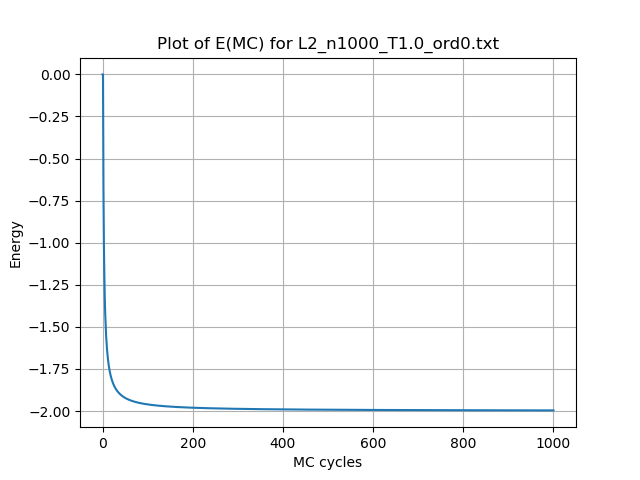
\includegraphics[width = 11cm]{img/energy_L2_n1000_T10_ord0.png}
      \caption{Energy-plot as function of MC-cycles. The lattice is $2 \times 2$ with 1000 Monte Carlo cycles and temperature 1.0. The spins are unordered. }
      \label{fig:energy_L2_n1000_T1.0_ord0}
    \end{figure}

  \begin{figure}[ht]
      \centering
      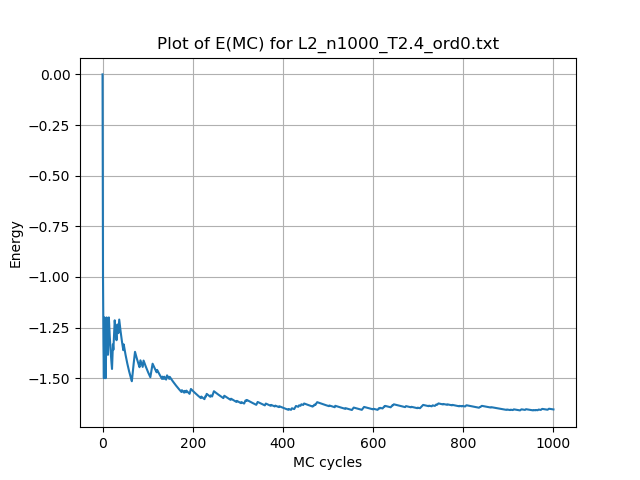
\includegraphics[width = 11cm]{img/energy_L2_n1000_T24_ord0.png}
      \caption{Energy-plot as function of MC-cycles. The lattice is $2 \times 2$ with 1000 Monte Carlo cycles and temperature 2.4. The spins are unordered. }
      \label{fig:energy_L2_n1000_T2.4_ord0}
    \end{figure}

  \begin{figure}[ht]
      \centering
      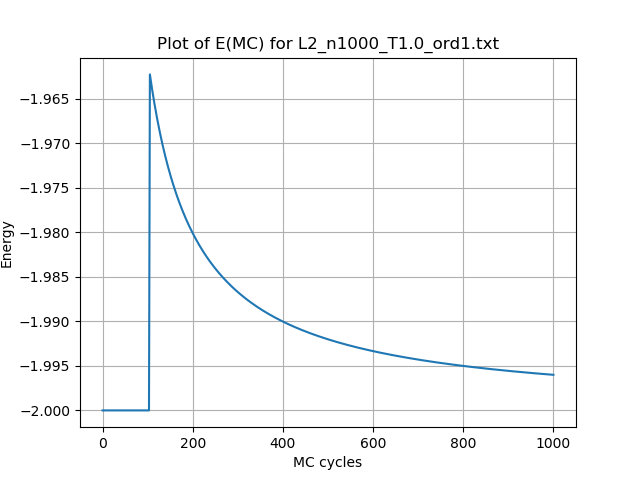
\includegraphics[width = 11cm]{img/energy_L2_n1000_T10_ord1.png}
      \caption{Energy-plot as function of MC-cycles. The lattice is $2 \times 2$ with 1000 Monte Carlo cycles and temperature 1.0. The spins are ordered. }
      \label{fig:energy_L2_n1000_T1.0_ord1}
    \end{figure}

  \begin{figure}[ht]
      \centering
      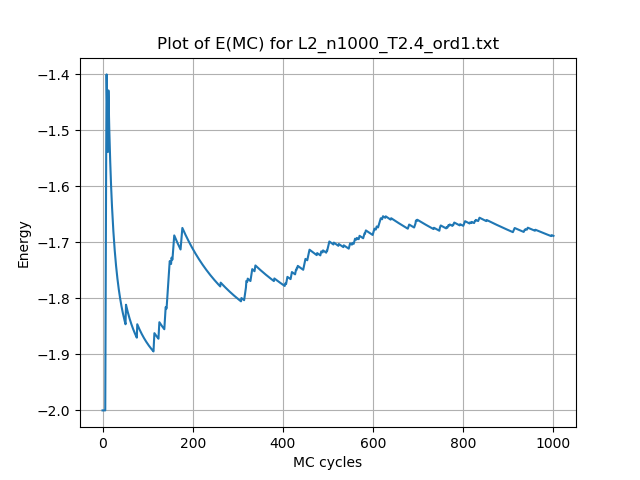
\includegraphics[width = 11cm]{img/energy_L2_n1000_T24_ord1.png}
      \caption{Energy-plot as function of MC-cycles. The lattice is $2 \times 2$ with 1000 Monte Carlo cycles and temperature 2.4. The spins are ordered. }
      \label{fig:energy_L2_n1000_T2.4_ord1}
    \end{figure}

\subsection{\texorpdfstring{ $20 \times 20$ }{text}-lattice} \label{sec:20x20lattice}

\subsubsection{Convergence-rate} \label{sec:convergence}

The energy and magnetization-plots for a 20x20-lattice is shown below. These show roughly when the results converge to the most likely state. \\


    \begin{figure}[ht]
      \centering
      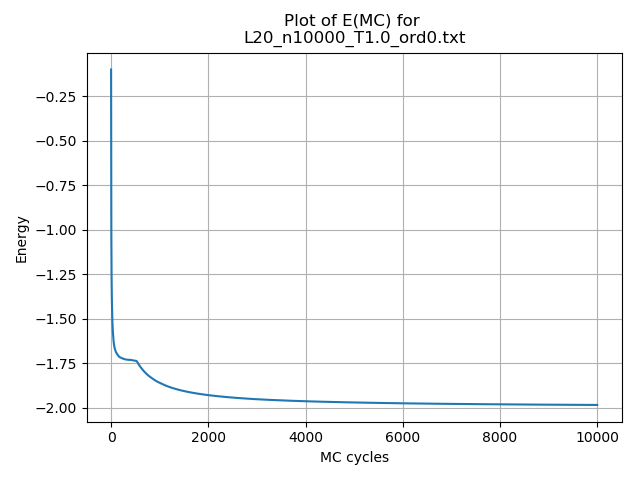
\includegraphics[width = 11cm]{img/energy_L20_n10000_T10_ord0.png}
      \caption{Energy-plot with low temperature and unordered spin (L=20, n=10k).}
      \label{fig:L20-energy-lowT-ord0}
    \end{figure}

    \begin{figure}[ht]
      \centering
      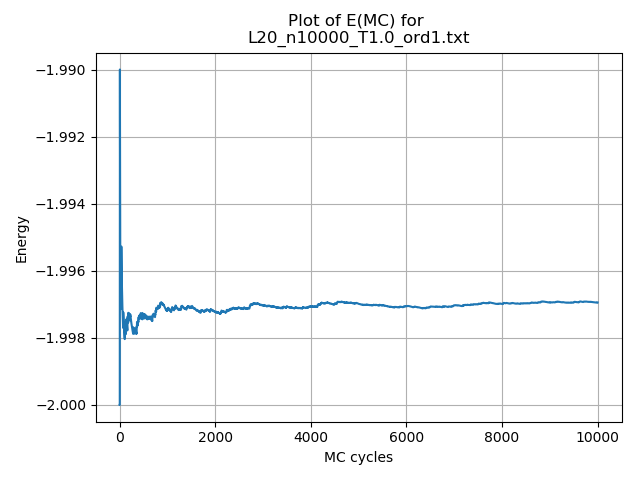
\includegraphics[width = 11cm]{img/energy_L20_n10000_T10_ord1.png}
      \caption{Energy-plot with low temperature and ordered spin (L=20, n=10k).}
      \label{fig:L20-energy-lowT-ord1}
    \end{figure}

    \begin{figure}[ht]
      \centering
      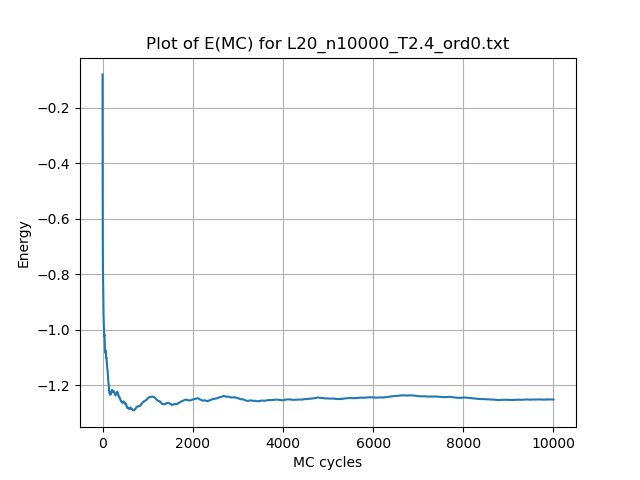
\includegraphics[width = 11cm]{img/energy_L20_n10000_T24_ord0.png}
      \caption{Energy-plot with high temperature and unordered spin (L=20, n=10k).}
      \label{fig:L20-energy-highT-ord0}
    \end{figure}

    \begin{figure}[ht]
      \centering
      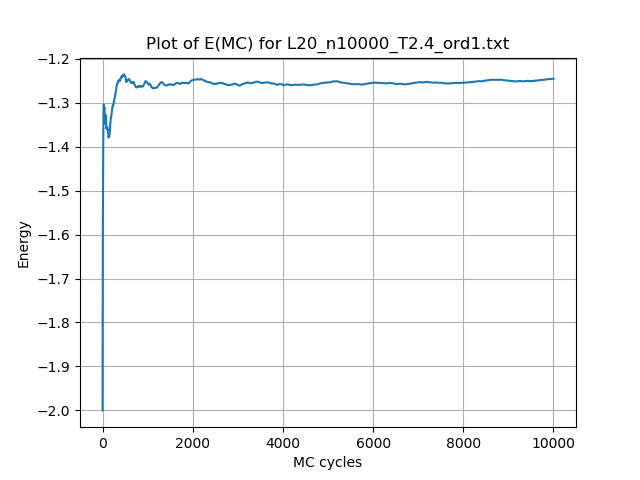
\includegraphics[width = 11cm]{img/energy_L20_n10000_T24_ord1.png}
      \caption{Energy-plot with high temperature and ordered spin (L=20, n=10k).}
      \label{fig:L20-energy-highT-ord1}
    \end{figure}

    \begin{figure}[ht]
      \centering
      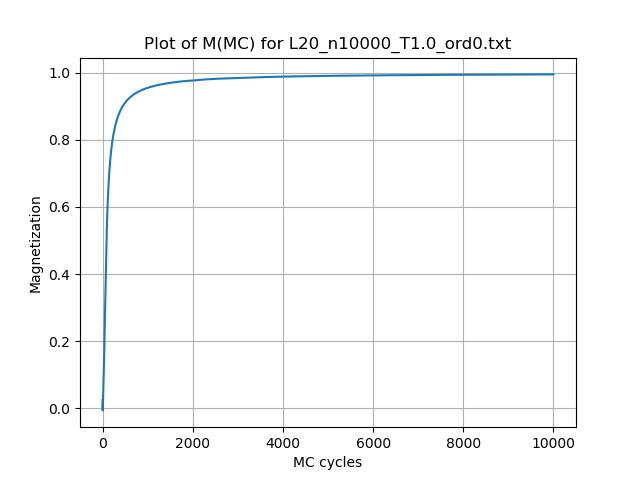
\includegraphics[width = 11cm]{img/magnet_L20_n10000_T10_ord0.png}
      \caption{Magnetization-plot with low temperature and unordered spin (L=20, n=10k).}
      \label{fig:L20-magnet-lowT-ord0}
    \end{figure}

    \begin{figure}[ht]
      \centering
      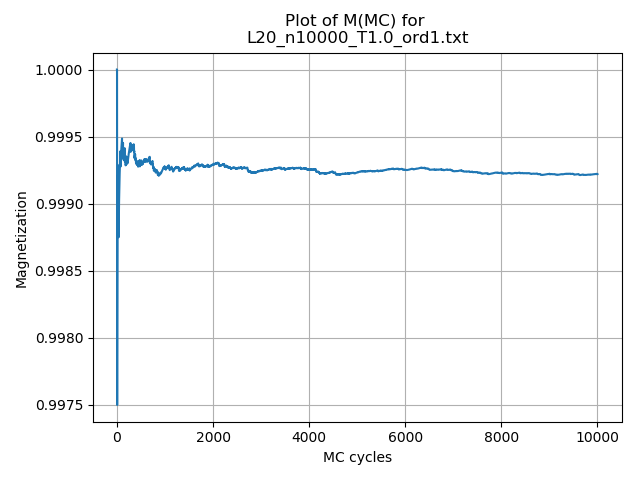
\includegraphics[width = 11cm]{img/magnet_L20_n10000_T10_ord1.png}
      \caption{Magnetization-plot with low temperature and ordered spin (L=20, n=10k).}
      \label{fig:L20-magnet-lowT-ord1}
    \end{figure}

    \begin{figure}[ht]
      \centering
      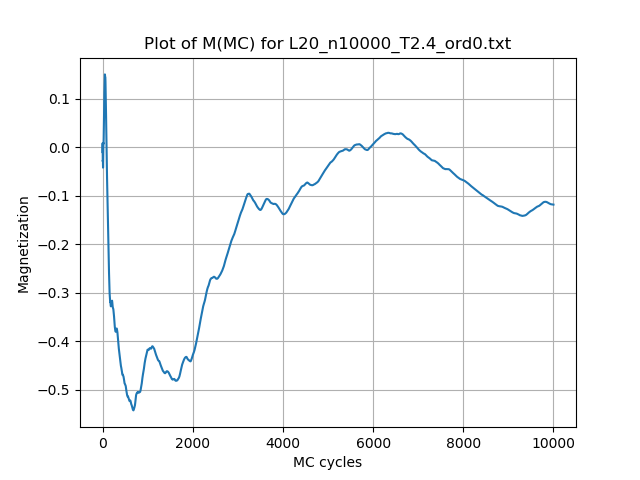
\includegraphics[width = 11cm]{img/magnet_L20_n10000_T24_ord0.png}
      \caption{Magnetization-plot with high temperature and unordered spin (L=20, n=10k).}
      \label{fig:L20-magnet-highT-ord0}
    \end{figure}

    \begin{figure}[ht]
      \centering
      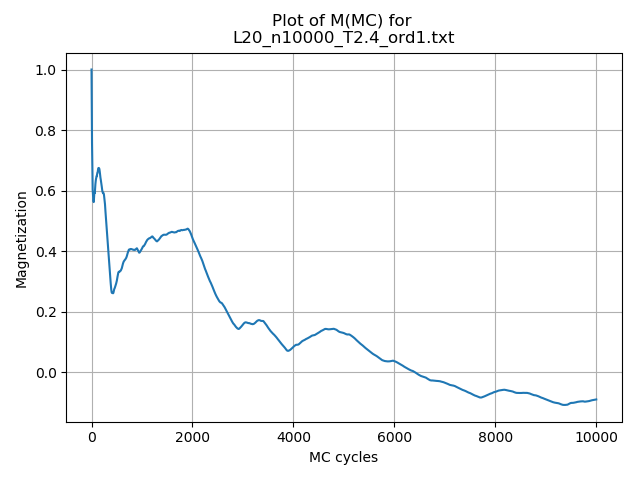
\includegraphics[width = 11cm]{img/magnet_L20_n10000_T24_ord1.png}
      \caption{Magnetization-plot with high temperature and ordered spin (L=20, n=10k).}
      \label{fig:L20-magnet-highT-ord1}
    \end{figure}


\subsubsection{Acceptance of spins} \label{sec:acceptance}

The following figures shows the number of accepted spins for each Monte Carlo cycle. This is how many spins are accepted to be flipped by the Metropolis algorithm. The figures are (\ref{fig:accept_L20_n10000_T1.0_ord0}), (\ref{fig:accept_L20_n10000_T1.0_ord1}), (\ref{fig:accept_L20_n10000_T2.4_ord0}) and (\ref{fig:accept_L20_n10000_T2.4_ord1}). \\

  \begin{figure}[ht]
      \centering
      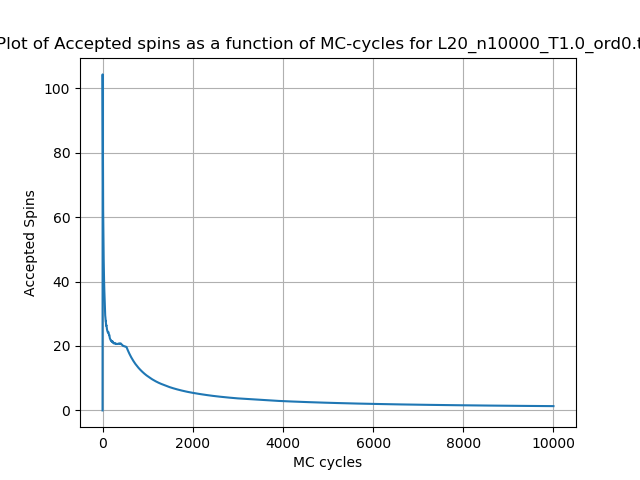
\includegraphics[width = 11cm]{img/accept_L20_n10000_T10_ord0.png}
      \caption{Cumulative acceptance per MC-cycle for 10000 Monte Carlo cycles with temperature 1.0. The spins are unordered. }
      \label{fig:accept_L20_n10000_T1.0_ord0}
    \end{figure}

  \begin{figure}[ht]
      \centering
      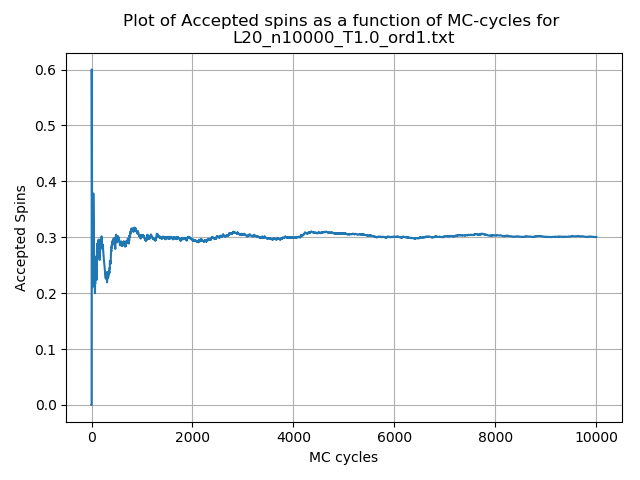
\includegraphics[width = 11cm]{img/accept_L20_n10000_T10_ord1.png}
      \caption{Cumulative acceptance per MC-cycle for 10000 Monte Carlo cycles with temperature 1.0. The spins are ordered. }
      \label{fig:accept_L20_n10000_T1.0_ord1}
    \end{figure}

  \begin{figure}[ht]
      \centering
      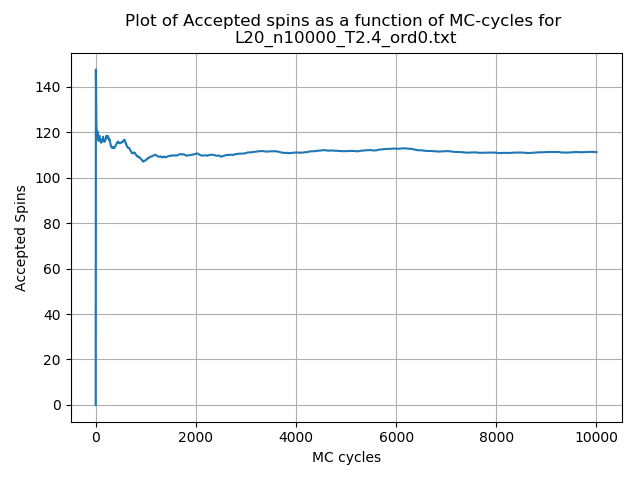
\includegraphics[width = 11cm]{img/accept_L20_n10000_T24_ord0.png}
      \caption{Cumulative acceptance per MC-cycle for 10000 Monte Carlo cycles with temperature 2.4. The spins are unordered. }
      \label{fig:accept_L20_n10000_T2.4_ord0}
    \end{figure}

  \begin{figure}[ht]
      \centering
      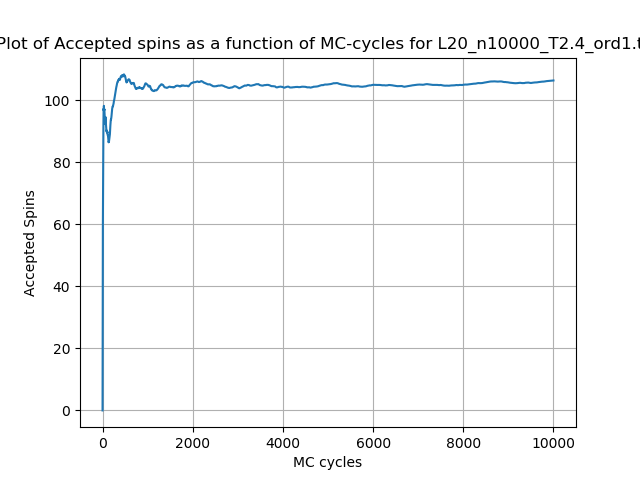
\includegraphics[width = 11cm]{img/accept_L20_n10000_T24_ord1.png}
      \caption{Cumulative acceptance per MC-cycle for 10000 Monte Carlo cycles with temperature 2.4. The spins are ordered. }
      \label{fig:accept_L20_n10000_T2.4_ord1}
    \end{figure}

\subsubsection{Probability distributions} \label{sec:probabilitydistributions}

The following figures depicts the probability distributions of both low and high temperatures for unordered and ordered spins. The lattice used is $20 \times 20$ with 1000000 Monte Carlo cycles. The figures are (\ref{fig:prob-lowT-ord0}), (\ref{fig:prob-lowT-ord1}), (\ref{fig:prob-highT-ord0}) and (\ref{fig:prob-highT-ord1}). \\

  \begin{figure}[ht]
      \centering
      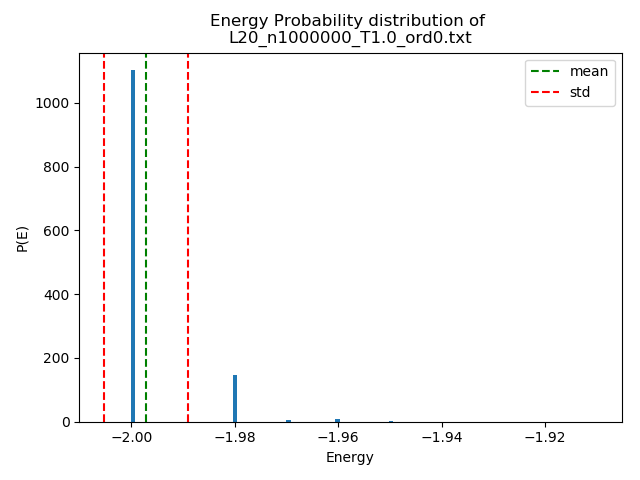
\includegraphics[width = 11cm]{img/energyhistogram_L20_n1000000_T10_ord0.png}
      \caption{Probability Distribution for low temperature with unordered spin (L=20, n=1mill).}
      \label{fig:prob-lowT-ord0}
    \end{figure}

  \begin{figure}[ht]
      \centering
      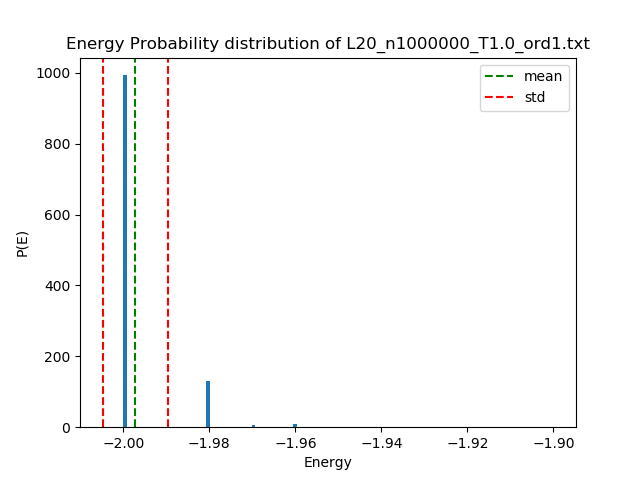
\includegraphics[width = 11cm]{img/energyhistogram_L20_n1000000_T10_ord1.png}
      \caption{Probability Distribution for low temperature with ordered spin (L=20, n=1mill).}
      \label{fig:prob-lowT-ord1}
    \end{figure}

  \begin{figure}[ht]
      \centering
      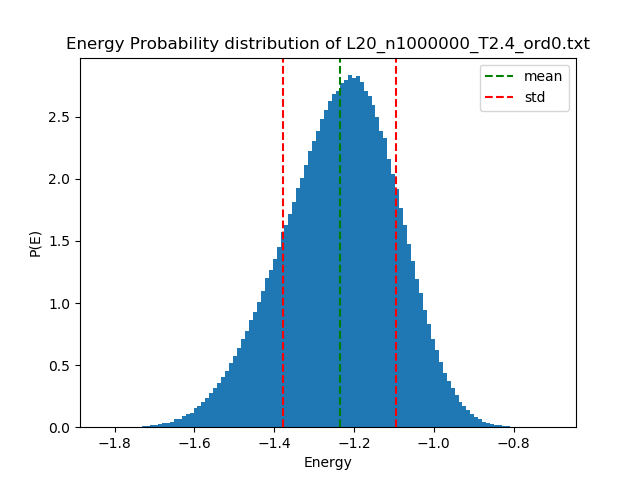
\includegraphics[width = 11cm]{img/energyhistogram_L20_n1000000_T24_ord0.png}
      \caption{Probability Distribution for high temperature with unordered spin (L=20, n=1mill).}
      \label{fig:prob-highT-ord0}
    \end{figure}

  \begin{figure}[ht]
      \centering
      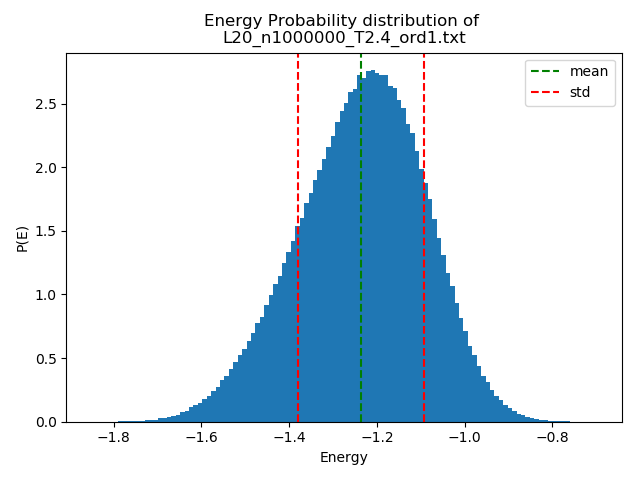
\includegraphics[width = 11cm]{img/energyhistogram_L20_n1000000_T24_ord1.png}
      \caption{Probability Distribution for high temperature with ordered spin (L=20, n=1mill).}
      \label{fig:prob-highT-ord1}
    \end{figure}


\subsection{Phase transition} \label{sec:phasetransition}

The following figures are depicting the variation of energy, specific heat, mean magnetization and susceptibility as a function of temperature for the four lattice sizes $40 \times 40$, $60 \times 60$, $80 \times 80$ and $100 \times 100$. The temperature is given in the interval $T = [2.0 , 2.3]$ with the step size 0.005. The number of Monte Carlo cycles is 100000. The figures are
(\ref{fig:tempvsenergy2}), (\ref{fig:tempvsspecitifheat2}), (\ref{fig:tempvsmeanmagnetization2}) and (\ref{fig:tempvssusceptibility2}).


  \begin{figure}[ht]
      \centering
      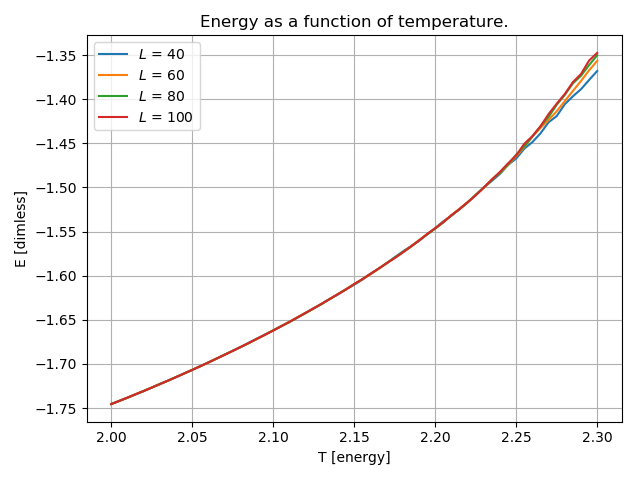
\includegraphics[width = 11cm]{img/tempvsenergy2.png}
      \caption{Energy as a function of temperature for 1000000 Monte Carlo cycles.}
      \label{fig:tempvsenergy2}
    \end{figure}

  \begin{figure}[ht]
      \centering
      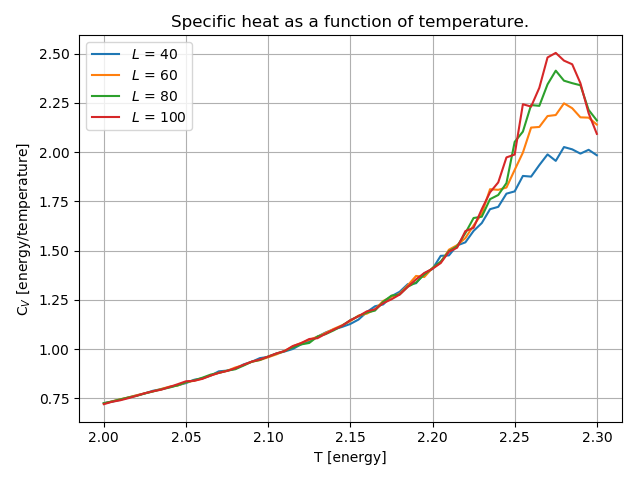
\includegraphics[width = 11cm]{img/tempvsspecificheat2.png}
      \caption{Specific heat as a function of temperature for 1000000 Monte Carlo cycles.}
      \label{fig:tempvsspecitifheat2}
    \end{figure}

  \begin{figure}[ht]
      \centering
      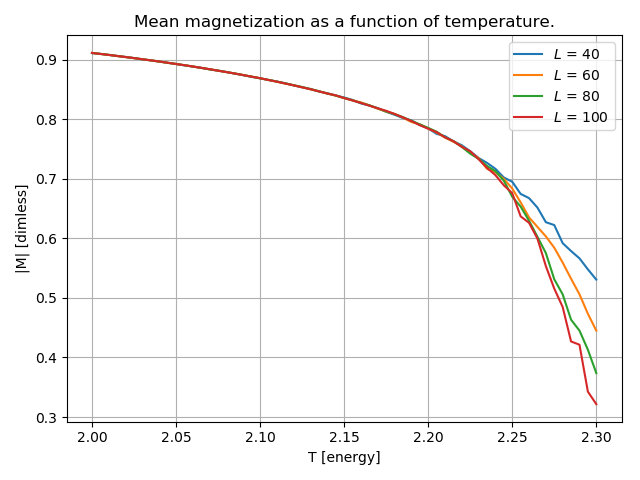
\includegraphics[width = 11cm]{img/tempvsmeanmagnetization2.png}
      \caption{Mean magnetization as a function of temperature for 1000000 Monte Carlo cycles.}
      \label{fig:tempvsmeanmagnetization2}
    \end{figure}

  \begin{figure}[ht]
      \centering
      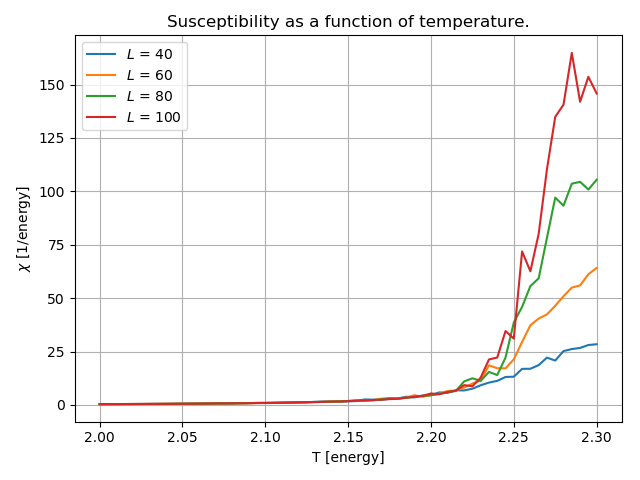
\includegraphics[width = 11cm]{img/tempvssusceptibility2.png}
      \caption{Susceptibility as a function of temperature for 1000000 Monte Carlo cycles.}
      \label{fig:tempvssusceptibility2}
    \end{figure}


\subsection{Critical temperature} \label{sec:criticaltemperature}

  The critical temperature for the different simulations is as shown in table (\ref{tab:critical}).

    \begin{table}[ht]
      \centering
      \caption{Critical temperature for simulations}
      \vspace{2mm}
      \label{tab:critical2}
      \begin{tabular}{|c|c|}
          \hline
           L & $T_c$\\
          \hline \hline
          40 & 2.280 \\
          60 & 2.280 \\
          80 & 2.275 \\
          100 & 2.275 \\
          \hline
      \end{tabular} \\
      \hspace{0pt}\\
    \end{table}

  To avoid $a=0$, the $100 \times 100$ -lattice will be compared with the $60 \times 60$ -lattice (case 1), and the $80 \times 80$ -lattice with the $40 \times 40$ -lattice (case 2). \\

  For case 1 the $a$-value is given as:

  $$(T_c(L_{100})-T_c(L_{60}))\cdot(L_{100}-L_{60})=a$$

  $$a=(2.275-2.280)\cdot(100-60)=-\frac{1}{5}=-0.2$$ \\

  For case 2, $a$ will also be $-0.2$.

  $$T_c(L=\infty)=\frac{a}{L}-T_c(L)$$ \\

  For case $L=100$:

  $$T_c(L=\infty)=\frac{-0.2}{100}-2.275$$ \\

  Following the same structure for each $L$ the following results are gotten. See table (\ref{tab:critical2}).

    \begin{table}[ht]
      \centering
      \caption{Critical temperature using \cite{onsager}}
      \vspace{2mm}
      \label{tab:critical}
      \begin{tabular}{|c|c|}
          \hline
           L & $T_c(L=\infty)$\\
          \hline \hline
          40  & 2.2850 \\
          60  & 2.2833 \\
          80  & 2.2775 \\
          100 & 2.2770 \\
          onsager & 2.269 \\
          \hline
      \end{tabular} \\
      \hspace{0pt}\\
    \end{table}
\fi

%--------------- Discussion ---------------------------------------
\vspace{1cm}

\clearpage
\newpage

\section{Discussion} \label{sec:Discussion}

\iffalse
Comparing the \texorpdfstring{ $2 \times 2$ }{text}-lattice's numerical values with the analytical ones we see there is an overall good correlation. See table (\ref{tab:analyticalvsnumerical}).\\

The expectation value for the energy is more or less identical. The same goes for the heat capacity and the expectation value for the absolute magnetization.\\

However, the susceptibility is quite a ways off.
This is quite unnerving. However, after many hours of debugging and re-checking analytical expressions, no reason was found, and as such the results have been left like that. The reason for this error could be from numerical errors, truncation errors hidden somewhere, faulty expressions or other similar explanations.\\

Looking at the file  \href{https://github.com/Erikbgram/Fys3150/blob/master/Project\%204/program/output/L2_n1000_T1.0_ord0.txt}{L2\_n1000\_T1.0\_ord0.txt} under output, one can see the general output-data for each MC iteration. This shows where the data starts fitting with the analytical values. The data in table (\ref{tab:analyticalvsnumerical}) used data from iteration 997 as this was the first with 3 decimal points of precision for $<E>$. It takes roughly 1000 MC-cycles for the numerical to start fitting with the analytical.

Looking at the graphs for the energy states with 10.000 Monte Carlo cycles we can see that the energy states quite quickly reaches an equilibrium state. between 2000 and 4000 has an extremely little variance of less than 0.0005. With the value ranging from roughly -1.997 and -1.9968. To later flatten ought an roughly -1.997.This shows that for the L=20 system it is more than enough with 10.000 Monte Carlo cycles for accurate data. \\

The same goes for the magnetization. At 10.000 an equilibrium state is once again reached roughly at around 4000 cycles, with a magnetization value of roughly 0.99925. \\

For $T=2.4$ the energies more or less the same result will be reached for 10.000 MC cycles. As one can see from the graphs above they both flatten ought at the roughly energy of -1.26. Unless extreme precision is needed 10.000 MC cycles should be enough to find the energy equilibrium state. \\

However, this is not true for the magnetization. For 10.000 MC cycles there is no real equilibrium state reached that is observable. Looking at the plot it would be hard to estimate a time where equilibrium is reached. To see clearer one would need plot with a higher amount MC-cycles. For 1.000.000 cycles, it's easier too see, and it converges around 400.000 cycles. This, however, is not central for our project, and for especially interested, one can look at the GitHub. \cite{github}. \\


For the probability distribution, 1.000.000 MC-cycles were used, and the evaluation of the distribution started at n=10.000. This was to make sure equilibrium was already reached.\\

Looking at the probability distributions for L=20 we found them pretty sensible at higher temperatures. For low temperatures they did not look very good. This is most likely attributed to the fact that low temperatures makes the metropolis algorithm less likely to accept a spin-flip, leading to fewer changes. The energies are more stable and as such only a few peaks exist. See figures (\ref{fig:accept_L20_n10000_T1.0_ord0}) - (\ref{fig:accept_L20_n10000_T2.4_ord1}). \\

Comparing the variance with the probability distributions we will ignore the $T=1.0$-plots as they are not that much to evaluate. For table (\ref{fig:accept_L20_n10000_T2.4_ord0} and (\ref{fig:accept_L20_n10000_T2.4_ord1}) the variance is $\approx0.02$ after equilibrium. This might sound weird, but since the figure couldn't be normalized properly (see program/probability\_distribution\_new.py for code) this could make sense. The plot is pretty steep, meaning most of the data is located around the mean (as can be seen in the figure). This means that the system seems to be very centered around the equilibrium after reaching it. In other words, it doesn't fluctuate that much. Looking at the near-end of the figures for L20 this is not hard to be convinced of.\\

Evaluating the actual shape of the distribution one can easily think it's a normal or possibly Gaussian distribution. In fact, the system should follow the Boltzmann distribution, as it is a simulation of a thermodynamical system. This is most likely easier to see for higher lattice-sizes. When comparing temperature differences this should also be easier to spot. \\

%--------------------------------------------------------

Looking at the final plots comparing the different $L$-values' specific heat, an indication of a phase transition can be found, see figures (\ref{fig:tempvsenergy2}), (\ref{fig:tempvsspecitifheat2}), (\ref{fig:tempvsmeanmagnetization2}) and (\ref{fig:tempvssusceptibility2}).
There is a large change in the data observed around $T=2.25$ for all lattices, and this would be due to a change in the structure, namely a phase transition. \\

The running time for this portion of the study was exceptionally long for all lattices, especially for $100 \times 100$. Therefore it would be smart to implement parallellization for our code, however parallellization made the program not faster at all. It made the program slower. For instance for the $40 \times 40$ - lattice
without parallellization, but with -O3 optimization, the time spent was 5423.37 seconds, while with parallellization the time spent was a whooping 32639 seconds. It is therefore understandable why we decided to not use parallellization on our program. For comparison the $80 \times 80$ - lattice with -O2 optimization in QT used 23355.5 seconds, the $60 \times 60$ - lattice with same conditions used 13416.1 seconds. The $100 \times 100$ - lattice run on a mac with -O3 compiler flag ran with 34462 seconds, which is slightly slower than a lattice 2/5 as small. The reason why the parallellized code is slower has not been found, after examining the two codes closely and thoroughly. The two codes should be exactly the same, only differing in the parallellization. \\


%----------------------------------------------------------


Studying the critical temperature we found the results to be reasonable. Due to a fixed step-length L40 and L60 had the same estimated $T_c$. The same went for L80 and L100. This was interesting, but not unlikely. One would think that increasing the lattice by that much would change the result, but it was pretty close. Had the results been smoothed out with least squares or something of the sort, a different number would have been found. However, this could easily be less accurate. When using \cite{task}'s Eq. (3), and calculating the $a$-value the final results were made. See table (\ref{tab:critical2}). \\

L100 was the closest, as it should and was 0.008 higher than Onsager's result was \cite{onsager}. This is pretty good.
Though increasing the lattice size further would lead to extremely slow calculations, we assume this would quickly converge to Onsager's value. \\
\fi

%---------------Conclusion and perspective---------------------------
\vspace{1cm}

\section{Conclusion and perspective} \label{sec:Conclusion}

\iffalse
In this project we have studied the convergence rate using the Ising model, evaluated the acceptance, and seen how the probability distribution looks. We also looked into the point in which phase transition occurs. This was calculated by use of equations from \ref{sec:criticaltemp}. This combined with simulations of the lattice with different sizes gave an approximated value. The results show that the phase transition occured around $T=2.27$ (scaled of course).
\fi

%----------------References----------------------------------------

\vspace{1cm}

\section{References} \label{sec:References}

\begin{thebibliography}{}

\iffalse
\bibitem{task}
Morten H. Jensen (2019), \href{https://github.com/CompPhysics/ComputationalPhysics/blob/master/doc/Projects/2019/Project4/pdf/Project4.pdf}{Project 4}, Departement of Physics, University of Oslo, Norway

\bibitem{github}
Erik B. Grammeltvedt, Alexandra Jahr Kolstad, Erlend T. North (2019), \href{https://github.com/Erikbgram/Fys3150}{GitHub}, Students of Departement of Physics, University of Oslo, Norway

\bibitem{lecture_slides}
Morten H. Jensen (2015), \href{https://github.com/CompPhysics/ComputationalPhysics/blob/master/doc/Lectures/lectures2015.pdf}{Lecture slides for FYS3150}, Department of Physics, University of Oslo, Norway

\bibitem{onsager}
Onsager (1944), \href{https://journals.aps.org/pr/abstract/10.1103/PhysRev.65.117}{"A Two-Dimensional Model with an Order-Disorder Transition"}, American Physical Society

\bibitem{isingmodel}
Jacob Linder (2018), \href{https://snl.no/Ising-modellen}{Ising-modellen}, Store Norske Leksikon \\
\fi

\end{thebibliography}


%--------------Appendix---------------------------------------------
\vspace{1cm}


\appendix
\section{Appendix} \label{sec:Appendix}

\iffalse
\subsection{Derivation of analytical formulae}

To derive the analytical formulae we need to know the hyperbolic functions cosh and sinh, and their correlation to the exponential function. \\

They are as follows

\begin{align*}
    2 \cosh (x) &= e^x + e^{-x} \\
    2 \sinh (x) &= e^x - e^{-x}
\end{align*} \\


\subsubsection{Derivation of the partition function} \label{sec:derivationpartitionfunction}

The partition function is introduced in section \ref{sec:partitionfunction}. \\

Deriving the equation.

\begin{align*}
  Z &= \sum_{i=1} ^{M} e^{- \beta E_i} = \sum_{i=1} ^{16} e^{- \beta E_i} \\
  &= 1 \cdot e^{- \beta (-8J)} + 4 \cdot e^{- \beta (0J)} + 2 \cdot e^{- \beta (8J)} + 4 \cdot e^{- \beta (0J)}
  + 4 \cdot e^{- \beta (0J)} + 1 \cdot e^{- \beta (-8J)} \\
  &= e^{8 \beta J} + 4 + 2 \cdot e^{-8 \beta J} + 4 + 4 + e^{8 \beta J} \\
  &= 2 e^{8 \beta J } + 2 e^{-8 \beta J} + 12 \\
  &= 2 \left( e^{8 \beta J} + e^{- 8 \beta J} \right) + 12 \\
  &= 2 \left( 2 \cosh(8 \beta J) \right) + 12 \\
  &= 4 \cosh(8 \beta J) + 12
\end{align*} \\


\subsubsection{Derivation of the expectation values of the energies} \label{sec:derivationenergies}

The expectation value of the energy is introduced in section \ref{sec:energyandmagnetization}. \\

Deriving the equation.

\begin{align*}
  \langle E \rangle &= \frac{1}{Z} \sum _{i=1} ^M E_i e^{- \beta E_i} \\
  &= \frac{1}{Z} \left[ 1 \cdot (-8J) e^{- \beta (-8J)} + 4 \cdot 0 + 2 \cdot (8J) e^{- \beta (8J)} + 4 \cdot 0 + 1 \cdot (-8J) e^{- \beta (-8J)} \right] \\
  &= \frac{1}{Z} \left[ - 8J e^{\beta 8J} + 2 \cdot 8J e^{- \beta 8J} - 8J e^{ \beta 8J} \right] \\
  &= \frac{2}{Z} \left[ - 8J e^{\beta 8 J} + 8 J e^{- \beta 8 J} \right] \\
  &= - \frac{16 J}{Z} \left( e^{8 \beta J} - e^{- 8 \beta J} \right) \\
  &= - \frac{16 J}{Z} (2 \sinh(8 \beta J) ) \\
  &= - \frac{32 J}{Z} \sinh(8 \beta J)
\end{align*} \\

The expectation value of the energy squared is introduced in section \ref{sec:specificheat}. \\

Deriving the equation.

\begin{align*}
  \langle E^2 \rangle &= \frac{1}{Z} \sum _{i=1} ^M E_i^2 e^{- \beta E_i} \\
  &= \frac{1}{Z} \left[ 1 \cdot (-8J)^2 e^{- \beta (-8J)} + 4 \cdot 0 + 2 \cdot (8J)^2 e^{- \beta (8J)} + 4 \cdot 0 + 1 \cdot (-8J)^2 e^{- \beta (-8J)} \right] \\
  &= \frac{1}{Z} \left[ 64 J^2 e^{\beta 8J} + 2 \cdot 64 J^2 e^{- \beta 8J} + 64 J^2 e^{ \beta 8J} \right] \\
  &= \frac{2 \cdot 64 J^2}{Z} \left[ e^{\beta 8 J} + e^{- \beta 8 J} \right] \\
  &= \frac{128 J^2}{Z} (2 \cosh(8 \beta J) ) \\
  &= \frac{256 J^2}{Z} \cosh(8 \beta J)
\end{align*} \\


\subsubsection{Derivation of the expectation values of the magnetizations} \label{sec:derivationmagnetizations}

The expectation value of the magnetization is introduced in section \ref{sec:energyandmagnetization}. \\

Deriving the equation.

\begin{align*}
  \langle \mathcal{M} \rangle &= \frac{1}{Z} \sum _{i=1} ^M \mathcal{M}_i e^{- \beta E_i} \\
  &= \frac{1}{Z} \left[1 \cdot 4 e^{- \beta (-8J)} + 4 \cdot 2 e^{- \beta (0J)} + 2 \cdot 0 + 4 \cdot 0 + 4 \cdot (-2)
  e^{- \beta (0J)} + 1 \cdot (-4) e^{- \beta (-8J)} \right] \\
  &= \frac{1}{Z} \left[ 4 e^{\beta 8J} + 8 - 8 - 4 e^{ \beta 8J} \right] \\
  &= \frac{1}{Z} \cdot 0 \\
  &= 0
\end{align*} \\

The expectation value of the mean magnetization is introduced in section \ref{sec:energyandmagnetization}. \\

Deriving the equation.

\begin{align*}
    \langle | \mathcal{M} | \rangle &= \frac{1}{Z} \sum _{i=1} ^M |\mathcal{M}_i| e^{- \beta E_i} \\
    &= \frac{1}{Z} \left[1 \cdot |4| e^{- \beta (-8J)} + 4 \cdot |2| e^{- \beta (0J)} + 2 \cdot |0| + 4 \cdot |0| + 4 \cdot |-2|
    e^{- \beta (0J)} + 1 \cdot |-4| e^{- \beta (-8J)} \right] \\
    &= \frac{1}{Z} \left[ 4 e^{\beta 8J} + 8 + 8 + 4 e^{ \beta 8J} \right] \\
    &= \frac{1}{Z} \cdot 4 \left[ 2 e^{\beta 8J} + 4 \right] \\
    &= \frac{8}{Z} \left( e^{\beta 8J} + 2 \right) \\
\end{align*}

The expectation value of the magnetization squared is introduced in section \ref{sec:susceptibility}. \\

Deriving the equation.

\begin{align*}
  \langle \mathcal{M}^2 \rangle &= \frac{1}{Z} \sum _{i=1} ^M \mathcal{M}_i^2 e^{- \beta E_i} \\
  &= \frac{1}{Z} \left[1 \cdot 4^2 e^{- \beta (-8J)} + 4 \cdot 2^2 e^{- \beta (0J)} + 2 \cdot 0 + 4 \cdot 0 + 4 \cdot (-2)^2 e^{- \beta (0J)} + 1 \cdot (-4)^2 e^{- \beta (-8J)} \right] \\
  &= \frac{1}{Z} \left[ 16 e^{\beta 8J} + 16 + 16 + 16 e^{ \beta 8J} \right] \\
  &= \frac{1}{Z} \left[ 2 e^{8 \beta J} + 2 \right] \\
  &= \frac{32}{Z} \left( e^{8 \beta J} + 1 \right) \\
\end{align*}


\subsection{Extracting the critical temperature} \label{sec:criticaltemp}

In order to find the critical temperature we will use \cite{task}'s Eq. (3). It is shown below:
$$T_c(L)-T_c(L=\infty)=aL^{-1/\nu}$$
where $\nu=1$. This gives
$$T_c(L)-T_c(L=\infty)=\frac{a}{L}$$
In order to find $a$ we subtract the equation with different $L$-values.
$$T_c(L_{100})-T_c(L=\infty)=\frac{a}{L_{100}}$$
$$T_c(L_{80})-T_c(L=\infty)=\frac{a}{L_{80}}$$
Subtracting gives
$$T_c(L_{100})-T_c(L_{80})=\frac{a}{L_{100}-L_{80}}$$
$$(T_c(L_{100})-T_c(L_{80}))\cdot(L_{100}-L_{80})=a$$ \label{eq:finding-a}
\fi

%\clearpage


%----------------Slutten av dokumentet---------------------------------------


%\end{multicols}

\end{document}
